\documentclass[a4paper, 12pt]{article}
\usepackage[latin1]{inputenc}
\usepackage[T1]{fontenc}
\usepackage[french]{babel}
\usepackage{graphicx}
\usepackage{amsmath}
\usepackage{amssymb}
\usepackage{hyperref}
\usepackage{listings}
\usepackage{color}


\definecolor{dkgreen}{rgb}{0,0.6,0}
\definecolor{gray}{rgb}{0.5,0.5,0.5}

\lstset{
	frame = tb,
	language = Caml,
	aboveskip = 3mm,
	belowskip = 3mm,
	showstringspaces = false,
	columns = flexible,
	basicstyle = {\small\ttfamily},
	numberstyle = \color{blue},
	keywordstyle = \color{red},
	commentstyle = \color{gray},
	stringstyle = \color{dkgreen},
	breaklines = true,
	breakatwhitespace = true,
	tabsize = 4
}

\pagestyle{headings}

\title{Rapport \\
Projet : programmation fonctionnelle}
\author{Quentin Januel \& Cl�ment Defr�ti�re}
\date{\today}

\begin{document}

\maketitle

\newpage
\section{Tests}

\subsection{Listes courtes}
% 

\subsection{Listes longues}
% 

\subsection{Listes d�j� tri�es}
% 

\newpage
\section{Analyse de complexit�}

Nous allons � pr�sent analyser le temps que prend chaque fonction de tri en fonction de la longueur de la liste qu'on lui passe en argument, en nous basant directement sur le code source de chacune des trois fonctions de tri. \\

Pour ce faire, nous allons d'abord consid�rer que ce temps est proportionnel au nombre de calculs que doit faire tel algorithme en fonction de la longueur de la liste. \\

Ainsi, pour une liste de taille $N$, nous recherchons l'ordre de grandeur en fonction de $N$ du nombre d'op�rations que va effectuer l'algorithme. \\ \\


Par soucis de simplification, nous allons consid�rer que les fonctions comme \texttt{List.length} ou \texttt @ sont instantann�es ou au moins proportionnelles � la longeur des listes avec lesquelles on les utilise. \\ \\


% Il est important de noter que, ne pouvant pas connaitre le temps exact des fonctions, nous ne recherchons que leur taux d'accroissement. \\ 

% Ce dernier est suffisant pour d�terminer quelle fonction sera la meilleure � partir d'une taille de listes suffisamment grande. \\ \\


Afin de repr�senter la complexit� d'un algorithme, nous allons utiliser la notation $O$. \\
Ainsi, un algorithme ayant une complexit� $O(n^2)$ sera un algorithme qui, pour une liste de taille $n$, effectue $n \times n$ op�rations (et prend donc un temps relativement proportionnel). \\ \\

Pour finir, nous n'allons pas prendre en compte les op�rations ne d�pendant pas de $n$, ni les facteurs multiplicatifs de $n$ puisque ces derniers n'auront aucun impact quand $n$ sera suffisamment grand. \\
Une complexit� $O(100+5 \times n)$ est donc la m�me que $O(n)$.

\newpage
\subsection{Tri par cr�ation du maximum}
% 

\newpage
\subsection{Tri par fusion}
Voici le code source de la fonction de tri par fusion : \\

\begin{lstlisting}
let rec tri_partition_fusion comp l =
	let l1, l2 = partitionne l in
		if (List.length l1)+(List.length l2) < 2 then
			l1@l2
		else
			let sorted1 = tri_partition_fusion comp l1
			and sorted2 = tri_partition_fusion comp l2 in
				fusionne comp sorted1 sorted2
;;
\end{lstlisting}

Nous pouvons constater que cette fonction fait elle m�me appel � deux fonctions ; \texttt{partitionne} et \texttt{fusionne}.
Ces derni�res ont toutes deux une complexit� $O(n)$. \\

A chaque �tape, cet algorithme coupe la liste en deux, pour ensuite les fusionner. \\
Nous pouvons le repr�senter par le diagramme ci dessous : \\

\begin{center}
	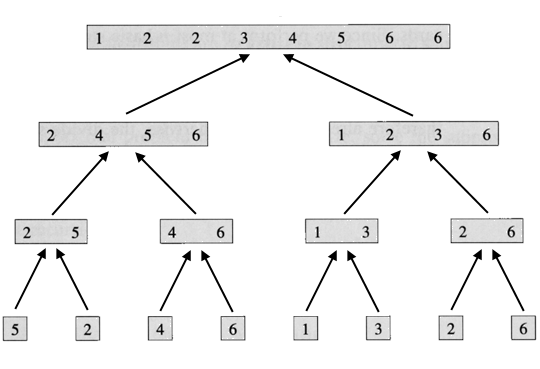
\includegraphics[scale=0.5]{mergesortDiagram.png}
\end{center}

Appelons niveau $i$ de l'algorithme la $i^{eme}$ ligne du sch�ma. \\

A chaque niveau, la liste est coup� en $p$ parties et la longueur de chaque sous liste est de $n/p$. Il y aura donc exactement $n$ calculs par niveau (puisque, rappelons le, \texttt{partitionne} et \texttt{fusionne} sont de complexit� $O(n)$). \\

La complexit� de cet algorithme est donc $O(n \times <\#niveaux>)$. \\
Le nombre de niveaux est le nombre de fois qu'il faut couper une liste en deux jusqu'� n'obtenir qu'un seul �l�ment. \\
Supposons que $n$ soit de la forme $2^a$, il y aura donc $a$ niveaux. \\
Plus g�n�ralement, pour une liste de longueur $n$, il y aura approximativement $log_{2}(n) = log(n)/log(2)$ niveaux. \\ \\

Cet algorithme a donc une complexit� $O(n \times ln(n))$.


\newpage
\subsection{Tri par arbre binaire de recherche}
% 


\newpage
\section{Comparaisons des courbes}


\newpage
\section{Bilan}




\end{document}

